% filepath: c:\Users\gabri\Documents\Ceub\tcc\sections\concepts.tex
\chapter{Conceitos}

\section{Fundamentos de Aerodinâmica}
A aerodinâmica é o ramo da física que estuda o comportamento do ar em movimento e sua interação com corpos sólidos, como asas e hélices de aeronaves. O entendimento dos fenômenos aerodinâmicos é fundamental para o projeto eficiente de aeronaves, influenciando diretamente o desempenho, a segurança e a eficiência energética \cite{anderson2017fundamentals}.

\begin{itemize}
    \item \textbf{Sustentação (\(L\))}: força perpendicular ao escoamento do ar, gerada pela diferença de pressão entre as superfícies superior e inferior do perfil aerodinâmico. É responsável por manter a aeronave em voo e depende da forma do perfil, do ângulo de ataque e das condições do escoamento \cite{anderson2017fundamentals}.
    \item \textbf{Arrasto (\(D\))}: força paralela e oposta ao movimento da aeronave, resultante da resistência do ar. O arrasto pode ser dividido em arrasto de forma, arrasto de fricção e arrasto induzido, sendo este último predominante em baixas velocidades e altos ângulos de ataque \cite{raymer2018aircraft}.
    \item \textbf{Eficiência aerodinâmica}: expressa pela razão \(C_L/C_D\), onde \(C_L\) é o coeficiente de sustentação e \(C_D\) o coeficiente de arrasto. Perfis com alta eficiência aerodinâmica proporcionam maior alcance e menor consumo de combustível \cite{abbott1959theory}.
\end{itemize}

Os coeficientes \(C_L\) e \(C_D\) são definidos por:
\[
C_L = \frac{L}{\frac{1}{2} \rho V^2 S}
\qquad
C_D = \frac{D}{\frac{1}{2} \rho V^2 S}
\]
onde \(\rho\) é a densidade do ar, \(V\) a velocidade relativa e \(S\) a área de referência.

Perfis de asas e hélices possuem funções distintas: as asas são projetadas para maximizar a sustentação e minimizar o arrasto em diferentes fases do voo (decolagem, cruzeiro), enquanto hélices convertem potência do motor em tração, transferindo energia para o ar e gerando força propulsora \cite{anderson2017fundamentals}. A otimização de asas normalmente considera decolagem e cruzeiro, pois o pouso envolve dispositivos hipersustentadores e condições operacionais específicas, com menor impacto no desempenho global.

As fases do voo — decolagem, cruzeiro e pouso — apresentam requisitos aerodinâmicos distintos. Na decolagem, busca-se máxima sustentação em baixas velocidades; no cruzeiro, prioriza-se eficiência e baixo arrasto; no pouso, a ênfase está na segurança e controle, frequentemente com uso intensivo de flaps e slats \cite{raymer2018aircraft}. Por isso, a otimização do pouso é usualmente excluída em estudos de desempenho global.

\section{Perfis Aerodinâmicos}
Perfis aerodinâmicos são seções transversais de asas ou hélices, cuja geometria determina o comportamento aerodinâmico do componente. O estudo detalhado dos perfis é fundamental para o projeto de aeronaves, pois influencia diretamente a geração de sustentação, o arrasto, a estabilidade e o controle.

A geometria de um perfil aerodinâmico é definida por parâmetros como corda, cambagem, espessura máxima, posição da espessura máxima, bordo de ataque e bordo de fuga. Cada um desses elementos exerce influência direta sobre o desempenho aerodinâmico, a eficiência estrutural e o comportamento em diferentes regimes de voo. Por exemplo, perfis com maior cambagem tendem a gerar mais sustentação, mas também apresentam maior arrasto, sendo indicados para fases de decolagem e manobra. Já perfis de baixa cambagem e menor espessura são preferidos para o cruzeiro, pois proporcionam menor arrasto e maior eficiência.

Além disso, a escolha do perfil afeta a estabilidade e o controle da aeronave. Perfis simétricos, cuja linha média coincide com a corda, são utilizados em superfícies de controle e hélices, pois não geram sustentação em ângulo de ataque nulo, facilitando o controle bidirecional. Perfis assimétricos, com cambagem positiva, são empregados em asas para maximizar a sustentação mesmo em baixos ângulos de ataque, aumentando a eficiência em voo de cruzeiro.

Outro aspecto importante é a influência dos dispositivos hipersustentadores, como flaps e slats, que modificam temporariamente a geometria do perfil para aumentar a sustentação em baixas velocidades. O uso desses dispositivos é fundamental para garantir operações seguras durante decolagens e pousos, permitindo que a aeronave opere em pistas mais curtas e com maior margem de segurança.

A análise dos perfis aerodinâmicos envolve a avaliação de suas polares, que relacionam o coeficiente de sustentação (\(C_L\)) ao coeficiente de arrasto (\(C_D\)) para diferentes ângulos de ataque. Essas curvas são essenciais para a seleção do perfil mais adequado a cada fase do voo e para a otimização do desempenho global da aeronave. Ferramentas computacionais como o XFOIL permitem simular o comportamento de diferentes perfis, considerando efeitos de Reynolds, transição laminar-turbulenta e presença de dispositivos móveis, fornecendo dados fundamentais para o processo de projeto e otimização.

\subsection{Partes de um Perfil Aerodinâmico}
Um perfil aerodinâmico é composto por diversas partes, cada uma com função específica:

\begin{itemize}
    \item \textbf{Bordo de ataque}: é a extremidade frontal do perfil, responsável por iniciar a separação do fluxo de ar. Seu formato influencia a resistência ao avanço e a tendência ao desprendimento do escoamento.
    \item \textbf{Bordo de fuga}: extremidade traseira do perfil, onde o fluxo de ar se reúne novamente. O ângulo e a espessura do bordo de fuga afetam o arrasto e a eficiência do perfil.
    \item \textbf{Linha média}: linha equidistante entre as superfícies superior e inferior do perfil, utilizada para definir a cambagem.
    \item \textbf{Superfície superior (extradorso)}: parte do perfil voltada para cima, geralmente associada à menor pressão devido à maior velocidade do escoamento.
    \item \textbf{Superfície inferior (intradorso)}: parte voltada para baixo, normalmente de maior pressão.
    \item \textbf{Corda (\(c\))}: distância linear entre o bordo de ataque e o bordo de fuga do perfil. É a referência para a maioria dos cálculos aerodinâmicos e influencia diretamente a geração de sustentação \cite{anderson2017fundamentals}.
    \item \textbf{Espessura máxima}: distância máxima entre o extradorso e o intradorso, importante para a resistência estrutural e o comportamento do escoamento.
    \item \textbf{Cambagem}: distância máxima entre a linha média do perfil e a corda. Perfis com maior cambagem tendem a gerar mais sustentação, porém com aumento do arrasto, sendo preferidos em asas de decolagem e manobra \cite{abbott1959theory}.
    \item \textbf{Espessura relativa}: razão entre a espessura máxima do perfil e a corda. Perfis mais espessos proporcionam maior resistência estrutural, mas podem aumentar o arrasto em regimes de alta velocidade \cite{anderson2017fundamentals}.
\end{itemize}

\begin{figure}[H]
    \centering
    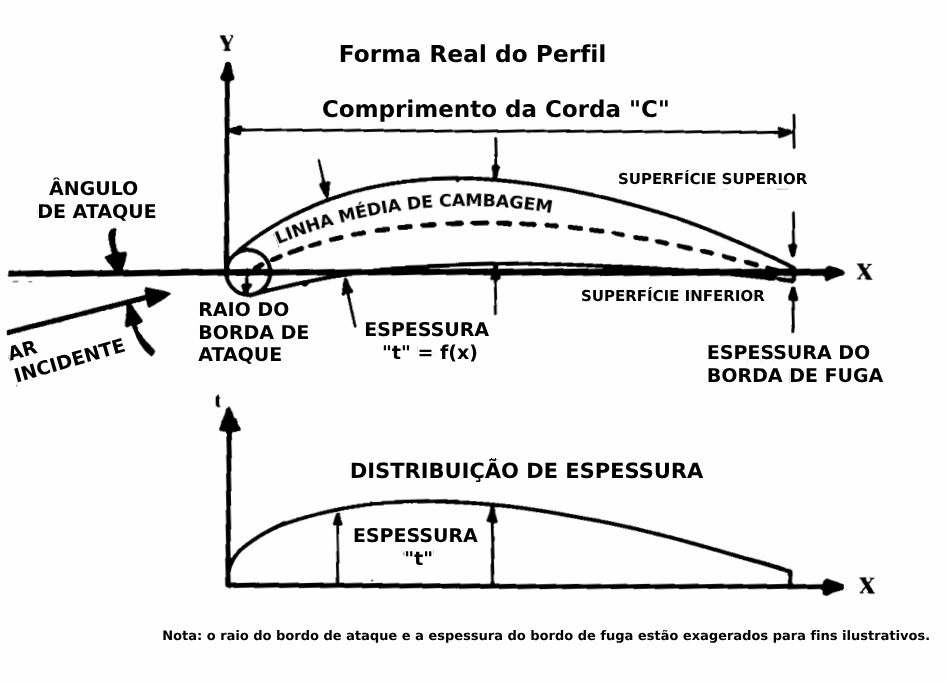
\includegraphics[width=0.6\textwidth]{figures/perfil_parametros.jpg}
    \caption{Exemplo de perfil aerodinâmico destacando corda, cambagem, espessura, bordo de ataque e bordo de fuga. \textbf{Fonte: Adaptado de \cite{raymer2018aircraft}}}
    \label{fig:perfil_parametros}
\end{figure}

\subsection{Tipos de Perfis}
Perfis podem ser classificados em simétricos e assimétricos. Perfis simétricos possuem linha média coincidente com a corda e são comuns em superfícies de controle e hélices, pois não geram sustentação em ângulo de ataque nulo. Perfis assimétricos (com cambagem) são preferidos em asas, pois geram sustentação mesmo em ângulos de ataque baixos, aumentando a eficiência em voo de cruzeiro.

A escolha do perfil aerodinâmico é fundamental para o desempenho da aeronave, pois afeta diretamente os coeficientes de sustentação (\(C_L\)) e arrasto (\(C_D\)), além da estabilidade e controle. Perfis de alta cambagem são indicados para decolagem e manobra, enquanto perfis de baixa cambagem e menor espessura são preferidos para cruzeiro, visando menor arrasto.

\subsection{Dispositivos Hipersustentadores: Flaps}
Flaps são dispositivos móveis instalados no bordo de fuga das asas, projetados para modificar temporariamente a geometria do perfil aerodinâmico. Quando defletidos, aumentam a curvatura (cambagem) e, consequentemente, a sustentação do perfil, permitindo operações seguras em baixas velocidades, como na decolagem e pouso. Durante o cruzeiro, os flaps são recolhidos para minimizar o arrasto e otimizar a eficiência \cite{raymer2018aircraft}.

Existem diversos tipos de flaps, cada um com características específicas:

\begin{itemize}
    \item \textbf{Flap simples}: consiste em uma única superfície articulada, fácil de projetar e operar, mas com aumento limitado de sustentação.
    \item \textbf{Flap dividido}: parte inferior do bordo de fuga é defletida, aumentando a sustentação e o arrasto, útil para pousos curtos.
    \item \textbf{Flap fendido}: possui uma fenda entre o flap e a asa, permitindo melhor escoamento e maior aumento de sustentação.
    \item \textbf{Flap Fowler}: além de defletir, se desloca para trás, aumentando a área da asa e a sustentação.
    \item \textbf{Flaps múltiplos}: combinações de flaps fendidos (duplo, triplo) para maximizar a sustentação em aeronaves de grande porte.
\end{itemize}

\begin{figure}[H]
    \centering
    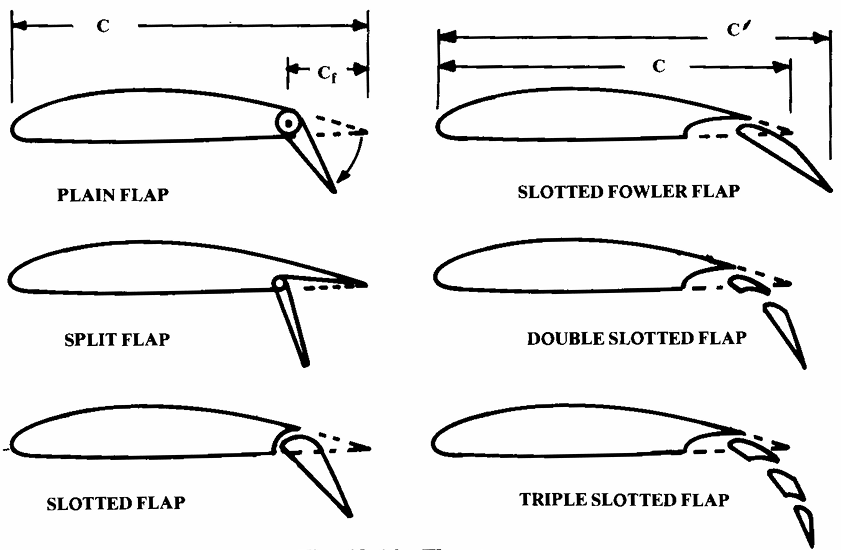
\includegraphics[width=0.6\textwidth]{figures/perfil_flap.png}
    \caption{Principais tipos de flaps utilizados em perfis aerodinâmicos: flap simples, flap dividido, flap fendido, flap Fowler fendido, flap duplo fendido e flap triplo fendido. Cada configuração proporciona diferentes aumentos de sustentação e controle durante pousos e decolagens. \textbf{Fonte: \cite{raymer2018aircraft}}.}
    \label{fig:perfil_flap}
\end{figure}

O uso de flaps altera significativamente a polar do perfil, elevando o coeficiente de sustentação máximo (\(C_{L_{max}}\)), mas também aumentando o arrasto. A análise detalhada dos perfis aerodinâmicos, incluindo a influência dos flaps e dos parâmetros geométricos, é essencial para a otimização do desempenho em diferentes fases do voo. Estudos clássicos, como os de Abbott e Von Doenhoff \cite{abbott1959theory}, fornecem bases experimentais e teóricas amplamente utilizadas até hoje.

\section{Corda Média Aerodinâmica (MAC)}
A corda média aerodinâmica (MAC, do inglês \textit{Mean Aerodynamic Chord}) é um conceito fundamental para o projeto e análise de asas, especialmente quando a asa possui geometria não retangular. A MAC representa uma corda fictícia que, se aplicada à asa, teria o mesmo momento aerodinâmico e área que a asa real. Seu cálculo é essencial para determinar o centro de gravidade, o ponto de aplicação das forças aerodinâmicas e para análises de estabilidade longitudinal.

Para uma asa trapezoidal, a MAC pode ser calculada por:
\[
\text{MAC} = \frac{2}{3} c_\text{raiz} \frac{1 + \lambda + \lambda^2}{1 + \lambda}
\]
onde \(c_\text{raiz}\) é a corda na raiz da asa e \(\lambda\) é o afilamento (\(\lambda = c_\text{ponta}/c_\text{raiz}\)). O posicionamento do centro de gravidade em relação à MAC é um parâmetro crítico para a estabilidade e controle da aeronave.

\begin{figure}[H]
    \centering
    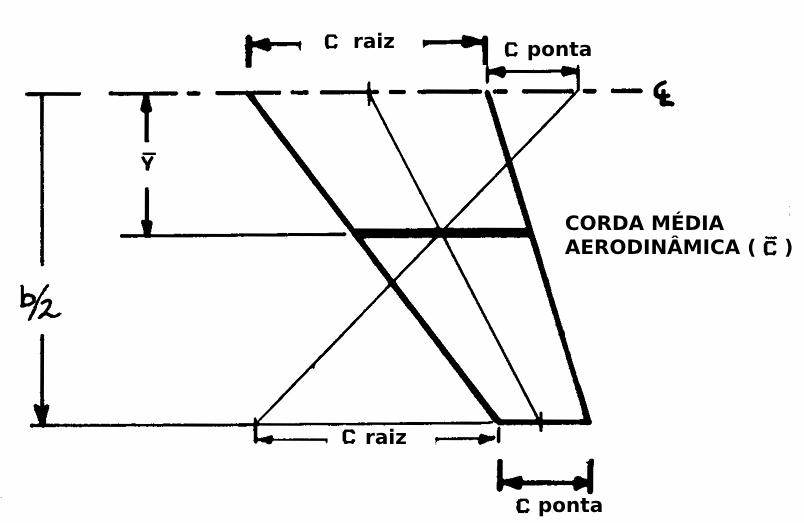
\includegraphics[width=0.7\textwidth]{figures/mac_trapezio.jpg}
    \caption{Representação esquemática da Corda Média Aerodinâmica (MAC) em uma asa trapezoidal, destacando as cordas na raiz e na ponta. \textbf{Fonte: Adaptado de \cite{raymer2018aircraft}}}
    \label{fig:mac_exemplo}
\end{figure}

A Figura~\ref{fig:mac_exemplo} ilustra de forma esquemática o conceito de Corda Média Aerodinâmica (MAC) em uma asa trapezoidal. Nela, é possível visualizar as cordas na raiz e na ponta da asa, bem como a posição e o comprimento da MAC, que representa a corda equivalente utilizada para cálculos de centro de gravidade, estabilidade e análise aerodinâmica. Essa representação facilita o entendimento da importância da MAC no contexto do projeto de asas com geometria não retangular.

\section{Razão de Aspecto}
A razão de aspecto (\(AR\), do inglês \textit{Aspect Ratio}) é definida como a razão entre o quadrado da envergadura (\(b\)) e a área da asa (\(S\)):
\[
AR = \frac{b^2}{S}
\]
Asas com alto AR (longas e estreitas) apresentam menor arrasto induzido e maior eficiência em voo de cruzeiro, sendo comuns em planadores e aeronaves de alta eficiência. Asas de baixo AR (curtas e largas) são mais manobráveis e resistentes, sendo utilizadas em caças e aeronaves de acrobacia. O AR influencia diretamente a distribuição de sustentação ao longo da envergadura e o comportamento do vórtice de ponta de asa.

\section{Software XFOIL}
O \textit{XFOIL} é um software amplamente utilizado para análise e projeto de perfis aerodinâmicos em regime sub-sônico. Desenvolvido por Mark Drela no MIT, o XFOIL combina métodos de escoamento potencial com modelagem detalhada da camada limite, permitindo a obtenção de polares de sustentação e arrasto, análise de estol, transição laminar-turbulenta e efeitos de Reynolds. O XFOIL é capaz de simular a influência de flaps, cambagem e espessura, sendo uma ferramenta essencial para engenheiros aeronáuticos e pesquisadores \cite{drela1989xfoil}.

Além disso, o XFOIL permite a exportação de dados para integração com algoritmos de otimização e inteligência artificial, acelerando o processo de seleção e ajuste de perfis para diferentes requisitos de missão.

\section{Inteligência Artificial: Fundamentos e Aplicações}
A inteligência artificial (IA) abrange técnicas computacionais que buscam simular a capacidade humana de aprender, adaptar-se e resolver problemas complexos. Em engenharia aeronáutica, a IA é empregada para otimização de formas, previsão de desempenho, análise de dados experimentais e automação de processos de projeto.

A aplicação da IA nesse contexto permite acelerar significativamente o desenvolvimento de aeronaves, reduzindo custos e tempo de projeto. Por meio de algoritmos inteligentes, é possível explorar grandes espaços de soluções, identificar padrões em dados experimentais e simular cenários que seriam inviáveis de serem testados fisicamente. Além disso, a IA contribui para a integração de diferentes áreas do conhecimento, como aerodinâmica, estruturas e controle, promovendo projetos mais eficientes e inovadores.

Entre as principais técnicas de IA utilizadas na engenharia aeronáutica destacam-se as redes neurais artificiais, os algoritmos evolutivos, as máquinas de vetor de suporte (SVM), árvores de decisão e métodos de aprendizado profundo (\textit{deep learning}). Essas técnicas podem ser aplicadas tanto na modelagem de fenômenos complexos, como o comportamento aerodinâmico de perfis e asas, quanto na otimização de parâmetros de projeto, seleção de materiais e análise de falhas.

No caso específico do projeto de perfis aerodinâmicos, a IA pode ser empregada para prever rapidamente os coeficientes de sustentação e arrasto a partir da geometria do perfil, substituir simulações demoradas por modelos preditivos, automatizar a busca por geometrias ótimas e até mesmo propor soluções inovadoras que não seriam facilmente encontradas por métodos tradicionais. A integração entre IA e ferramentas de simulação, como o XFOIL, potencializa ainda mais o processo de desenvolvimento, permitindo a avaliação de milhares de configurações em tempo reduzido.

Além disso, a IA tem papel fundamental na análise de dados experimentais, identificando tendências, anomalias e oportunidades de melhoria. Em projetos avançados, técnicas de aprendizado por reforço podem ser utilizadas para desenvolver sistemas autônomos de controle de voo, capazes de se adaptar a diferentes condições operacionais e otimizar o desempenho em tempo real.

Por fim, a adoção da inteligência artificial na engenharia aeronáutica representa uma tendência irreversível, impulsionando a inovação, a eficiência e a competitividade do setor. O domínio dessas técnicas torna-se cada vez mais essencial para engenheiros e pesquisadores que desejam atuar na fronteira do conhecimento e contribuir para o avanço da aviação.

\subsection{Redes Neurais Artificiais}
Redes neurais artificiais são modelos matemáticos inspirados no funcionamento do cérebro humano, compostos por camadas de neurônios artificiais interconectados. São capazes de aprender padrões complexos a partir de grandes volumes de dados, sendo amplamente utilizadas para:

\begin{itemize}
    \item Aproximação de funções não lineares (como polares aerodinâmicas).
    \item Previsão de coeficientes aerodinâmicos a partir de parâmetros geométricos.
    \item Redução do custo computacional em simulações, substituindo modelos físicos por modelos preditivos.
    \item Otimização multiobjetivo, quando combinadas com algoritmos evolutivos.
\end{itemize}

As redes podem ser do tipo \textit{feedforward} (mais comuns em regressão e classificação) ou recorrentes (para séries temporais). O treinamento é realizado por algoritmos como retropropagação do erro (\textit{backpropagation}), utilizando grandes bases de dados geradas por simulações ou experimentos.

\subsection{Algoritmos Evolutivos}
Algoritmos evolutivos são métodos de otimização inspirados nos processos de seleção natural e evolução biológica. Entre os principais estão os algoritmos genéticos, estratégias evolutivas e programação genética. Suas principais características incluem:

\begin{itemize}
    \item Operação sobre populações de soluções, promovendo diversidade e evitando mínimos locais.
    \item Uso de operadores como seleção, cruzamento (crossover) e mutação para explorar o espaço de soluções.
    \item Aplicação em problemas de múltiplos objetivos e restrições não lineares, comuns em projetos aeronáuticos.
    \item Integração com simulações (como XFOIL) para avaliação automática de milhares de geometrias de perfis.
\end{itemize}

Esses algoritmos são especialmente úteis quando o espaço de busca é vasto e pouco conhecido, permitindo encontrar soluções inovadoras e eficientes.

\subsection{Sinergia entre IA e Otimização}
A combinação de redes neurais e algoritmos evolutivos potencializa o processo de otimização: redes neurais podem ser treinadas para prever rapidamente o desempenho de novos perfis, enquanto algoritmos evolutivos exploram o espaço de soluções em busca de geometrias ótimas. Essa abordagem híbrida reduz drasticamente o tempo de projeto e permite a análise de soluções que seriam inviáveis por métodos tradicionais.